\chapter{Preliminaria matematyczne}\label{ch:02}

\section{Wprowadzenie}\label{sec:intromat}

Odwrócone wahadło to przykład wahadła, które środek swojej masy ciężkości ma powyżej punktu obrotu, przez co jest układem wysoce niestabilnym. Układ taki charakteryzuje się dwoma punktami swobody: punkt obrotu pręta i poruszający się poziomo wózek, oraz tylko jednym wejściem sterującym, które odpowiada za ruch poziomy układu. Problem polega na takim sterowaniu wózkiem w osi poziomej, aby wahadło było utrzymane w osi pionowej, bądź oscylowało wokół punktu równowagi, bez opadania w dół. Sterowanie odbywa się poprzez przykładanie siły tylko do wózka, na wahadło działała tylko siła grawitacji i jej składowe, a jego punkt obrotu jest w pełni swobodny. 

\section{Model matematyczny} \label{sec:modelmat}

Układ odwróconego wahadła został przedstawiony na rysunku \ref{fig:draw}. Rzeczywisty układ wahadła uwzględnia moment bezwładności pręta, który w tym modelu został zastąpiony przez pręt o pomijalnie małej masie i niewielkiej masie \textit{m} na jego końcu. 

\begin{figure}
    \centering
    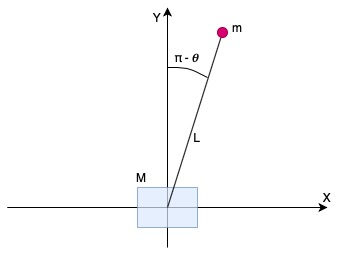
\includegraphics[scale=0.8]{praca_dyplomowa_wzor/figures/pendulum_draw.jpg}
    \caption{Układ odwróconego wahadła}
    \label{fig:draw}
\end{figure}

Współrzędne końca wahadła są opisane przez:
\begin{equation}
    \begin{cases}
    x_{p}=x+L\sin{\Theta}\\ 
    y_{p}=L\cos{\Theta}
    \end{cases}
\end{equation}
gdzie \textit{x} to współrzędna masy \textit{M}. Składowe prędkości masy \textit{m} można wyznaczyć przez pierwsze pochodne jego współrzędnych: 
\begin{equation}
    \begin{cases}
    \dot{x}_{p}=\dot{x}+L\dot{\Theta}\cos{\Theta}\\
    \dot{y}_{p}=-L\dot{\Theta}\sin{\Theta}
    \end{cases}
    \label{skladowe}
\end{equation}

Energia kinetyczna kinetyczna układu może być wyrażone przez równanie \ref{ekin}, przy założeniu, że ramię wahadła ma pomijalnie małą masę, a tym samym jego moment bezłwadności jest równy 0.
\begin{equation}
    K=\frac{1}{2}M{v_{1}}^{2}+\frac{1}{2}m{v_{2}}^{2},
    \label{ekin}
\end{equation}
gdzie \textit{v\textsubscript{1}} i \textit{v\textsubscript{2}} to odpowiednio prędkosci mas \textit{M} i \textit{m} i wynoszą:
\begin{equation}
    \begin{array}{l}
         v_1=\dot{x} \\
         v_2=\sqrt{\dot{x_p}^{2}+\dot{y_p}^{2}}
    \end{array}
\end{equation}
Korzystajac z wyprowadzenia \ref{skladowe} kwadrat prędkość \textit{v\textsubscript{2}} mozna wyraznić następujaco: 
\begin{equation}
    v_2^2=(\dot{x}+L\dot{\Theta}cos(\Theta))^{2}+(-L\dot{\Theta}sin(\Theta))^{2}=\dot{x}^2+2L\dot{\Theta}\dot{x}\cos{\Theta}+L^2\dot{\Theta}^2
\end{equation}
Zatem energia kinetyczna układu jest równa:
\begin{equation}
    K=\frac{1}{2}(M+m)\dot{x}^2+mL\dot{\Theta}\dot{x}\cos{\Theta}+\frac{1}{2}mL^2\dot{\Theta}^2
\end{equation}
,,Energia potencjalna układu pochodzi od siły grawitacji działającej na kulę" \cite{TchMu18} i wyraża się wzorem:
\begin{equation}
    V=mgL\cos{\Theta}
\end{equation}

Łącząc wyprowadzone równania na energię kinetyczną i potencjalną otrzymamy lagranżian:

\begin{equation}
    L=K-V=\frac{1}{2}(M+m)\dot{x}^2+mL\dot{\Theta}\dot{x}\cos{\Theta}+\frac{1}{2}mL^2\dot{\Theta}^2-mgL\cos{\Theta}
\end{equation}

Do wyznaczenia równań Eulera-Lagrange’a potrzebne są następujące pochodne:
\begin{equation}
        \begin{array}{l}
         \frac{\partial L}{\partial x}=0 \\ \\
         \frac{\partial L}{\partial \Theta}=mg\sin{\Theta} \\ \\
         \frac{\partial L}{\partial \dot{x}}=(M+m)\dot{x}+mL\dot{\Theta}\cos{\Theta} \\ \\
         \frac{\partial L}{\partial \dot{\Theta}}=mL\dot{x}\cos{\Theta}+mL^2\dot{\Theta}
    \end{array}
\end{equation}